\documentclass[a4paper,fleqn, review]{cas-sc}
\usepackage[numbers,sort&compress]{natbib}
\usepackage{graphicx}
\usepackage{booktabs}
\usepackage{multirow}
\usepackage{amsmath}
\usepackage{xcolor}
\usepackage{placeins}

\newcommand{\rev}[1]{\textcolor{red}{#1}}

\newcommand{\placeholderfig}[2][0.86\linewidth]{%
  \fbox{\parbox[c][3.4cm][c]{#1}{\centering\footnotesize\ttfamily
    [FIGURE PLACEHOLDER]\\[4pt]#2}}%
}

\begin{document}

\shorttitle{DBR-Net for road extraction}
\shortauthors{L.X. Thang et~al.}

\title[mode=title]{DBR-Net: A Gated Dual-branch Network with Centerline
Supervision for Road Extraction from High-resolution Remote Sensing Imagery}

%% Authors
\author[1,2]{Le Xuan Thang}[type=editor,
	auid=000,bioid=1,
	orcid=0000-0002-9911-3544]
\ead{lexuanthang.official@outlook.com}
\ead[url]{https://lexuanthang.vn}

\author[1,2]{Giang Tuan Hung}[type=editor,
	auid=000,bioid=1,
  orcid=0009-0000-1313-4516]
\ead{hunggl@civix.com.vn}

\author[2]{Vu Manh Trung}[type=editor,
	auid=000,bioid=1,
	orcid=0009-0009-7596-1520]
\ead{trung211101196@lms.utc.edu.vn}

\author[2]{Tran Ngoc Hoa}[type=editor,
	auid=000,bioid=1,
	orcid=0009-0005-9255-3263]
\cormark[1]
\ead{ngochoa@utc.edu.vn}

%% Corresponding author
\cortext[cor=1]{Corresponding author}

%% Affiliations
\affiliation[1]{
	organization={CIVIX - Civil Intelligence and eXpanded Data Company Limited},
	city={Hanoi},
	country={Vietnam}
}

\affiliation[2]{
	organization={Application of Artificial Intelligence for Structural Health Monitoring (AI-SHM) Research Group, Faculty of Civil and Environment Engineering (R2026-UTC-01), University of Transport and Communications},
	city={Hanoi},
	country={Vietnam}
}

\begingroup
\colorlet{originaltextblack}{black}
\colorlet{originalsectioncolor}{scolor}
\colorlet{originalheadingcolor}{hscolor}
\colorlet{black}{red}
\colorlet{scolor}{red}
\colorlet{hscolor}{red}
\color{red}
\begin{abstract}
Automatic road extraction from high-resolution satellite and aerial imagery
supports map updating, logistics planning, and post-disaster response. The task
remains difficult because road surfaces cover only a few percent of the pixels,
form thin and elongated structures that are frequently occluded by trees,
shadows, and vehicles, and are useful only when their connectivity is preserved.
Encoder-decoder networks that downsample deeply discard the evidence for narrow
roads before the decoder can recover it, whereas networks that hold high
resolution throughout are costly at inference time. This paper presents
DBR-Net (Dual-Branch Road Network), a segmentation network built around a detail
stream that never leaves stride~8 and a semantic stream that descends to
stride~32 to gather context. The two streams communicate through a single
bilateral exchange regulated by a zero-initialized spatial gate, so that the
network starts as an exact copy of an ungated residual exchange and acquires
selectivity gradually.
Broad context is aggregated by a progressive pyramid pooling module built on
group normalization and re-enters the detail stream through a controlled fusion
step. Connectivity is supervised by an auxiliary centerline head trained with an
asymmetric Tversky objective whose targets come from a pure-tensor morphological
thinning applied before any downsampling. Every multi-branch block fuses exactly
into a single convolution for deployment. On the Massachusetts Roads and
DeepGlobe benchmarks, evaluated at native resolution with Hann-weighted
sliding-window inference, the proposed network reaches a road IoU of
72.19\% and 61.76\%, respectively, exceeding the strongest baseline by
0.75 percentage points on both datasets while requiring 22.53~M parameters,
90.457~GFLOPs, and 3.99~GB of GPU memory for a $512\times512$ input.
\end{abstract}

\begin{keywords}
\color{red}
road extraction \sep semantic segmentation \sep remote sensing \sep
structural re-parameterization \sep global-local context \sep feature fusion
\end{keywords}

\maketitle
\color{red}

\section{Introduction}
\label{sec:introduction}

Road networks form a fundamental layer of geospatial information systems and
support applications such as map updating, logistics planning, and emergency
response. However, road maps can become outdated as construction, closures, and
damage alter the network faster than manual digitization can capture. The
increasing availability of high-resolution optical satellite and aerial imagery
makes automatic road extraction a practical means of updating this information
\rev{\cite{abdollahi2020roadreview,chen2022roadsurvey,luweng2025roadreview}}.
For many downstream applications, accurate road coverage is important, but so is
the continuity of the extracted network because even a short missing segment can
interrupt an otherwise valid route.

Road extraction is commonly formulated as binary semantic segmentation, but it
remains challenging for several reasons. Road pixels often occupy only a small
fraction of an image, which can bias pixel-wise learning toward the background
class. Roads are also thin, elongated structures whose visual evidence may be
weakened by repeated downsampling. Their appearance varies with surface material,
illumination, and acquisition conditions, while rivers, field boundaries,
rooftops, and other linear structures can produce similar local patterns.
Occlusion by trees, shadows, buildings, and vehicles introduces additional gaps
\rev{\cite{mnih2013aerial,cheng2017cascaded,zhou2020btroadnet}}. Consequently,
effective road extraction requires both fine spatial detail and broader semantic
context. Pixel-overlap metrics remain useful for evaluation, but they may
under-penalize small disconnections that are important to network usability.

Existing approaches address these challenges along two main directions.
Encoder--decoder models, including U-Net \cite{ronneberger2015unet}, Deep
Residual U-Net \cite{zhang2018resunet}, and D-LinkNet
\cite{zhou2018dlinknet}, recover spatial resolution through skip connections and
decoder stages. Later methods improve contextual representation through
non-local operations \cite{wang2022nllinknet}, multi-resolution exchange
\cite{wang2021hrnet}, or attention-based decoders
\cite{xie2021segformer,wang2022unetformer}. A complementary line of research
introduces geometric or connectivity-related supervision, including road
centerlines \cite{cheng2017cascaded,lu2019msmtre}, local direction
\cite{ding2021diresnet}, connectivity attention \cite{mei2021coanet}, and
topology-aware objectives \cite{oner2022connectivity,shit2021cldice}. Although
these developments improve road delineation, retaining high-resolution features
throughout a network can increase computation, whereas aggressive downsampling
can remove evidence for narrow roads. Multi-branch feature aggregation may also
improve optimization while adding inference-time cost. These trade-offs motivate
a design that preserves spatial detail selectively, incorporates contextual
information, and remains efficient after deployment.

To this end, we propose DBR-Net, an asymmetric dual-branch network for road
extraction. A detail stream remains at stride~8 to retain fine spatial evidence,
while a semantic stream reaches stride~32 to capture broader context. The two
streams communicate through a single bilateral exchange controlled by a
single-channel spatial gate. The final gate convolution is zero-initialized so
that the exchange initially behaves like its ungated residual counterpart and
learns spatial selectivity during training. A progressive pyramid pooling module
aggregates multi-scale context, and a controlled fusion module returns this
information to the detail stream. In addition, an auxiliary centerline head
encourages structural continuity. Its targets are generated before downsampling
using max-pooling-based morphological thinning, and the head is optimized with
an asymmetric Tversky loss that assigns a larger penalty to false-negative road
pixels than to false positives \cite{salehi2017tversky}. The multi-branch blocks
are structurally re-parameterized into single convolutions for deployment
\cite{ding2021repvgg}.

We evaluate DBR-Net on the Massachusetts Roads \cite{mnih2013aerial} and
DeepGlobe \cite{demir2018deepglobe} datasets. DBR-Net achieves road IoU scores
of 72.19\% and 61.76\%, respectively, exceeding the strongest compared baseline
by 0.75 percentage points on both benchmarks. The corresponding F1-scores are
84.02\% and 74.21\%. For a $512\times512$ input, the model contains 22.53~M
parameters, requires 90.457~GFLOPs, and uses 3.99~GB of GPU memory.

The main contributions of this work are summarized as follows:

\begin{enumerate}
\item We introduce an asymmetric dual-resolution architecture that retains a
      stride-8 detail stream and couples it to a context-oriented semantic stream
      through a single gated bilateral exchange.
\item We develop an auxiliary centerline-supervision scheme whose targets are
      generated by tensor-based morphological thinning before downsampling and
      optimized with an asymmetric Tversky objective to emphasize missed road
      pixels.
\item We combine the proposed representation with structurally
      re-parameterizable blocks and demonstrate a favorable accuracy--efficiency
      balance on two public road-extraction benchmarks.
\end{enumerate}

The remainder of this paper is organized as follows.
Section~\ref{sec:related-work} reviews road extraction architectures,
multi-resolution designs, connectivity supervision, and structural
re-parameterization. Section~\ref{sec:methods} presents the overall architecture
and each of its modules, followed by the training objective.
Section~\ref{sec:experimental-setup} specifies the datasets, splits, training
strategy, and metrics. Section~\ref{sec:results-discussion} reports the
comparison with prior work and the efficiency analysis.
Section~\ref{sec:conclusion} summarizes the findings, discusses the limitations,
and outlines directions for future work.

\section{Related work}
\label{sec:related-work}

\subsection{Encoder-decoder networks for road extraction}
\label{subsec:rw-encdec}

\rev{Mnih~\cite{mnih2013aerial} trained neural networks on large aerial image
datasets to label road pixels from a wide image context, because occlusions and
shadows cast by trees and tall buildings often make local cues insufficient, and
released the Massachusetts Roads dataset, which established} patch-based learning of road
masks from aerial imagery as a benchmark task. \rev{Fully convolutional
networks~\cite{shelhamer2017fcn}, trained end to end from pixels to pixels, then moved
segmentation from patch-wise classification to dense prediction over inputs of
arbitrary size.} U-Net
\cite{ronneberger2015unet} introduced the skip-connected encoder-decoder that
most later road models inherit: the encoder builds semantic capacity by
downsampling, and lateral skips return spatial detail to the decoder. Deep
Residual U-Net \cite{zhang2018resunet} \rev{rebuilt this architecture from
residual units} and reported improved road delineation on Massachusetts with fewer
parameters than the original.

The DeepGlobe challenge \cite{demir2018deepglobe} shifted attention to
0.5\,m/pixel satellite imagery and larger scene variety. Its winning entry,
D-LinkNet \cite{zhou2018dlinknet}, \rev{built on the LinkNet architecture with a
pretrained encoder,} inserted a cascade of
dilated convolutions at the encoder bottleneck, enlarging the receptive field
without an additional downsampling stage, and it remains the reference baseline
on that benchmark. \rev{NL-LinkNet \cite{wang2022nllinknet} added non-local
blocks to a LinkNet-based network, so that every location can draw on global
context, and outperformed D-LinkNet with 43\% fewer parameters.} The
shared limitation of this family is structural rather than incidental. Skip
connections return detail that survived the encoder, but a road eight to twenty
pixels wide is represented by a fraction of a pixel at stride 32, so what the
decoder receives through the deepest skips is context, not geometry. Dilation
mitigates the problem by avoiding one downsampling step; it does not remove the
dependence on a deeply downsampled trunk.

\subsection{Multi-resolution and dual-branch architectures}
\label{subsec:rw-multires}

A second design maintains high resolution throughout the network instead of
recovering it. HRNet \cite{wang2021hrnet} runs parallel branches at several
resolutions and repeatedly exchanges information among all of them, which keeps a
high-resolution representation available at every depth. The approach is
effective for position-sensitive tasks, but the exchange is dense: every pair of
resolutions is fused at every stage, and the cost grows with the number of
branches.

Real-time segmentation networks reduce that cost to two branches. BiSeNet~V2
\cite{yu2021bisenetv2} pairs a shallow detail branch with a deeper semantic
branch and merges them once through a guided aggregation layer. DDRNet
\cite{pan2023ddrnet} keeps two resolutions throughout and exchanges between them
repeatedly, and introduces the deep aggregation pyramid pooling module to enlarge
the receptive field at the low-resolution branch. \rev{Both were
developed for real-time scene parsing and benchmarked chiefly on street-level
scenes}, where objects are large and the detail branch mainly
sharpens boundaries. Overhead road imagery inverts that balance: the structures
of interest are themselves near the resolution limit, so which resolutions
exchange, and under what control, matters more than how many exchanges occur.
\rev{DDRNet sums projected features of the two branches without any gating, and
the guided aggregation layer of BiSeNet~V2 multiplies each branch by
sigmoid-activated responses of the other, a dense gate over every channel and
location rather than a single spatial map; neither} is initialized so that
adding the exchange leaves a pretrained encoder undisturbed. \rev{Within road
extraction, DBRANet \cite{chen2022dbranet} places a dual-branch module, a
residual block beside a refined asymmetric block, in the encoder of a U-shaped
network and decodes with a regional attention module; its two branches
strengthen the feature extraction of the encoder, and the network keeps the
encoder-decoder layout discussed in Section~\ref{subsec:rw-encdec}.}

Context aggregation modules developed for scene parsing are used across both
families. Pyramid pooling \cite{zhao2017pspnet} and atrous spatial pyramid
pooling \rev{\cite{chen2018deeplab}} both compute several receptive-field scales
in parallel and combine them once at the end. The deep aggregation variant
\cite{pan2023ddrnet} adds hierarchical residual connections among the pooling
branches. These modules are normally built on batch normalization, which becomes
unreliable at the small per-device batch sizes \rev{\cite{wu2020groupnorm}} that 1024-pixel remote sensing
crops impose, particularly for a branch that pools to a single spatial location.

\subsection{Connectivity and topology-aware supervision}
\label{subsec:rw-topology}

Because pixel overlap is insensitive to short breaks, a separate line of work
supervises connectivity explicitly. \rev{Several road networks predict the
centerline as a second task: CasNet \cite{cheng2017cascaded} cascades a
centerline extraction network onto a road detection network and thins its output
into a single-pixel-wide centerline network, RCNN-UNet \cite{yang2019rcnnunet}
and MSMT-RE \cite{lu2019msmtre} train road detection and centerline extraction
jointly in U-Net-based multi-task models, and RoadNet \cite{liu2019roadnet}
predicts road surfaces, edges, and centerlines simultaneously. DiResNet
\cite{ding2021diresnet} supervises local road directions at the pixel level and
adds a structural supervision and a refinement network to improve road
topology, and BT-RoadNet \cite{zhou2020btroadnet} refines a coarse road map with
a second encoder-decoder and uses a spatial context module to counter
discontinuities.} CoANet
\cite{mei2021coanet} matches the network to road geometry directly, using strip
convolutions along four directions together with a connectivity attention module
that predicts whether neighboring locations belong to the same road. \rev{A
further line abandons the raster mask and builds the road graph directly:
RNGDet \cite{xu2022rngdet} generates the road network graph vertex by vertex from
an aerial image with a transformer, motivated by the limited topological
correctness of segmentation-based approaches. The present work stays
within the raster formulation, whose consequences are discussed in
Section~\ref{sec:conclusion}.}

Loss functions attack the same problem without changing the architecture. Region
losses of the Dice family \cite{milletari2016vnet} and reweighted classification
losses \rev{\cite{lin2020focal}} counteract the imbalance itself, and the Tversky loss
\cite{salehi2017tversky} generalizes Dice with separate weights for false
positives and false negatives, so an application can declare which error is worse.
\rev{Oner et al.~\cite{oner2022connectivity} express road connectivity through
the background regions that a gap in the prediction wrongly merges, and penalize
such connections so that the gaps close.}
clDice \cite{shit2021cldice} measures overlap between the skeletons of prediction
and label, which makes a break expensive even when it costs few pixels, and
provides a differentiable soft skeletonization built from morphological
operations.

Two practical constraints in this literature motivate the present design. First,
skeleton-based supervision is often implemented with external morphological
libraries operating on CPU arrays, which complicates distributed training and
makes the target dependent on a library version. Second, when the auxiliary head
sits at a reduced stride, the natural implementation downsamples the label and
then thins it; that order merges narrow branches and intersections, which are
precisely the structures the term is meant to protect.

\subsection{Structural re-parameterization}
\label{subsec:rw-reparam}

Multi-branch blocks improve optimization but cost inference time. \rev{ACNet
\cite{ding2019acnet} strengthened square kernels with parallel one-dimensional
asymmetric convolutions during training and converted the trained network back
into its original architecture, so the added branches cost nothing at
inference.} RepVGG
\cite{ding2021repvgg} showed that a training-time block of parallel $3\times3$,
$1\times1$, and identity paths, each followed by batch normalization, can be
folded algebraically into a single $3\times3$ convolution, so the deployed model
is a plain sequential stack with no accuracy loss. The transformation is exact:
batch normalization folds into the preceding convolution, and kernels padded to a
common size sum linearly.

Re-parameterization has been applied mainly to classification backbones
\rev{\cite{ding2019acnet, ding2021repvgg}} and
general-purpose detectors. Its combination with a detail-preserving segmentation
design for remote sensing, where inference runs over thousands of overlapping
tiles per scene and branch-level memory traffic is a real cost, has to our
knowledge not been reported. The blocks used here follow the same algebra\rev{;
like ACNet, they} add
anisotropic $1\times5$ and $5\times1$ depthwise branches, chosen for the
elongated geometry of road segments \rev{in the spirit of the strip convolutions
of CoANet \cite{mei2021coanet}}, that fuse into a single $5\times5$ depthwise
kernel.

\colorlet{black}{originaltextblack}
\colorlet{scolor}{originalsectioncolor}
\colorlet{hscolor}{originalheadingcolor}
\color{black}
\endgroup

\section{Methodology}
\label{sec:methods}



\begingroup
\color{red}

\section{Experimental setup}
\label{sec:experimental-setup}
To demonstrate the effectiveness of our proposed architecture, we evaluate its performance on public road segmentation datasets, detailing the experimental setup, implementation specifics, and a comparative analysis against state-of-the-art methods.

\subsection{Datasets and preprocessing}
\label{subsec:datasets}

We benchmark DBR-Net on two public road extraction datasets:

- The Massachusetts Roads dataset \cite{mnih2013aerial} comprises 1,171 aerial images of Massachusetts, each with a spatial resolution of 1 m/pixel and a size of $1500 \times 1500$ pixels. Covering more than 2,600 km$^2$, the dataset is officially divided into 1,108 training, 14 validation, and 49 test images. The corresponding ground-truth road masks were derived from OpenStreetMap centerlines and rasterized using a line width of 7 pixels.

- The DeepGlobe Road Extraction dataset \cite{demir2018deepglobe} consists of 8,570 RGB satellite images acquired over diverse urban and rural regions in Thailand, Indonesia, and India. Each image has a size of $1024 \times 1024$ pixels and a spatial resolution of 0.5 m/pixel. Covering approximately 2,220 km$^2$, the dataset is divided into 6,226 training, 1,243 validation, and 1,101 test images. The ground-truth masks provide pixel-level binary annotations of the complete road surfaces rather than road centerlines, with road and background pixels represented as foreground and background classes, respectively.

Representative image--mask pairs from the Massachusetts Roads and DeepGlobe
datasets are shown in Fig.~\ref{fig:dataset-samples}.

\begin{figure}[pos=htbp]
  \centering
  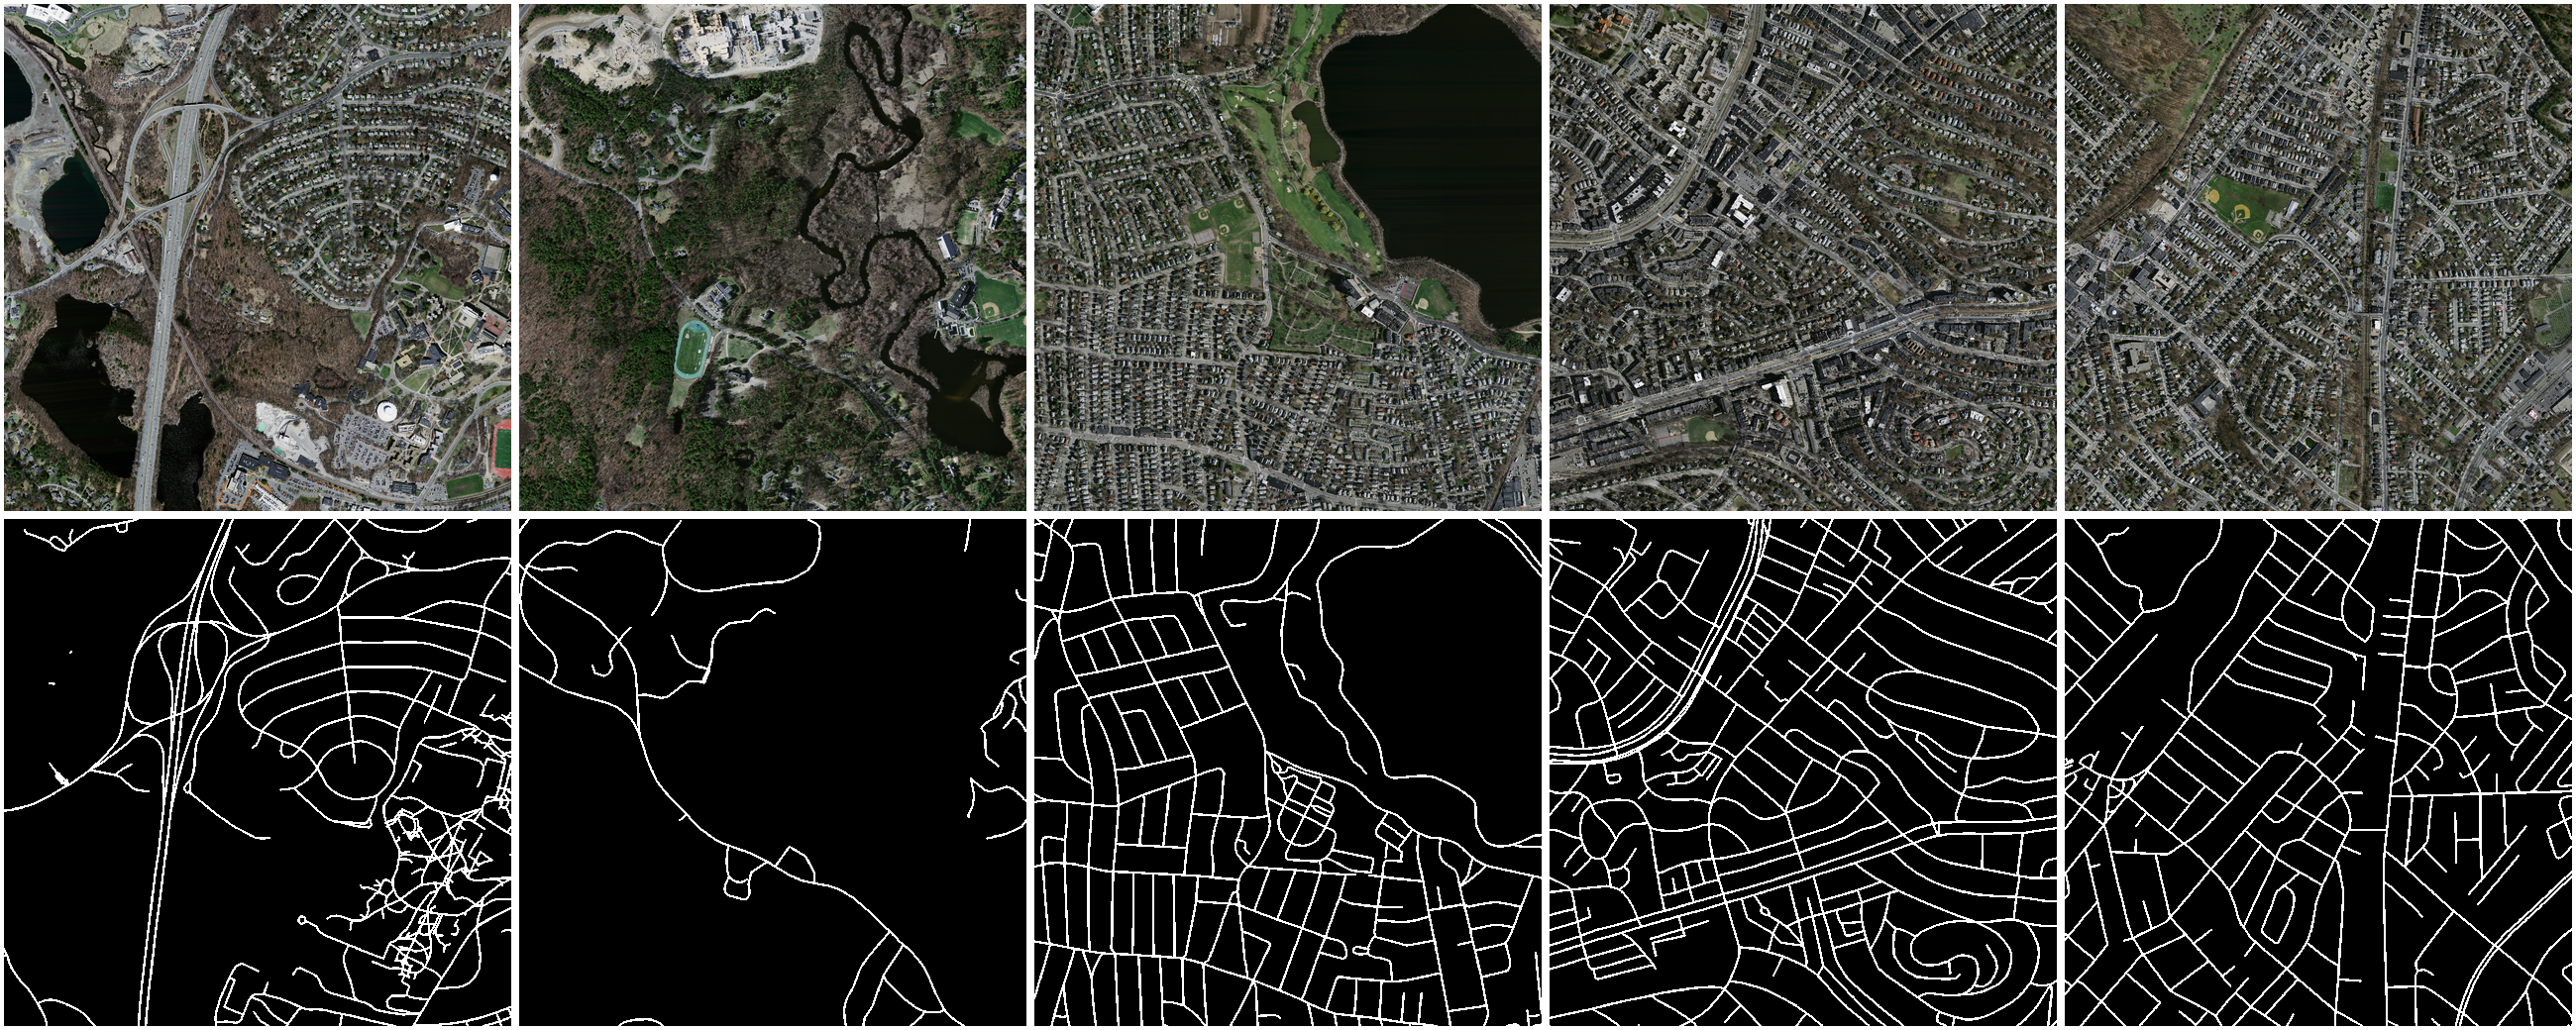
\includegraphics[width=\linewidth]{figs/massachusetts_samples_5x2.png}
  \par\smallskip
  \textbf{(a) Massachusetts Roads}
  \par\medskip
  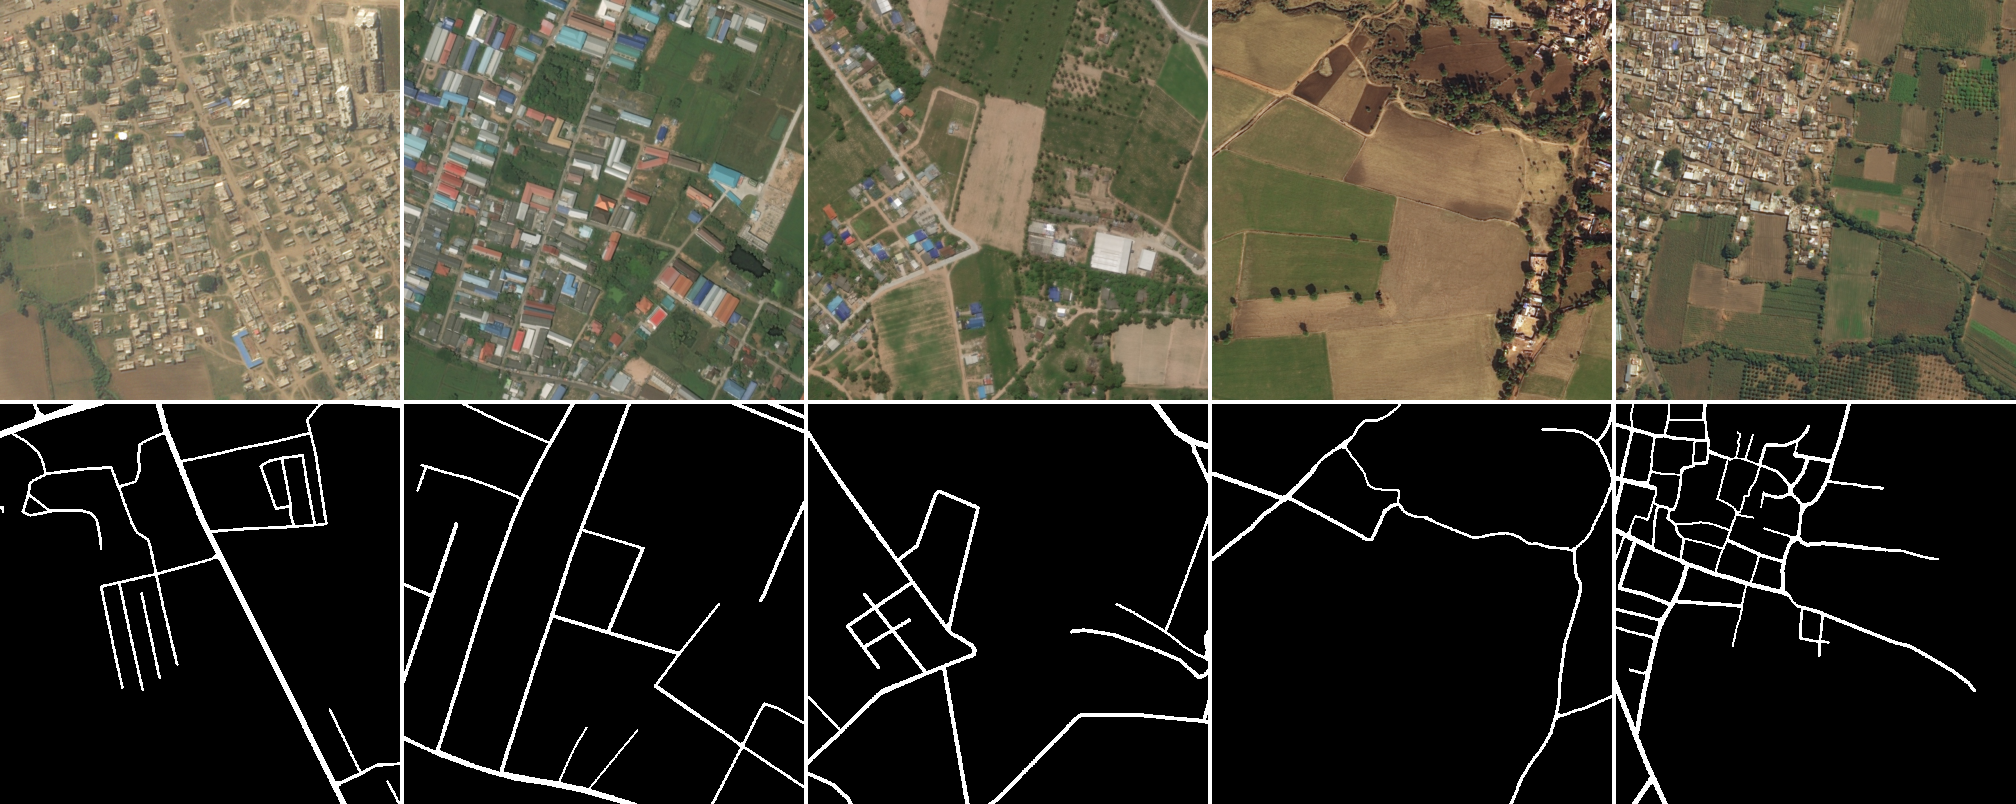
\includegraphics[width=\linewidth]{figs/deepglobe_samples_5x2.png}
  \par\smallskip
  \textbf{(b) DeepGlobe Road Extraction}
  \caption{Representative image--mask pairs from the two road-extraction
  datasets: (a) Massachusetts Roads and (b) DeepGlobe Road Extraction. For
  each dataset, the top row shows the input images and the bottom row shows
  the corresponding ground-truth road masks.}
  \label{fig:dataset-samples}
\end{figure}
\FloatBarrier

\subsection{Implementation details}
\label{subsec:implementation}

All experiments were conducted on a workstation running 64-bit Windows 11 Pro,
equipped with two Intel Xeon Gold 6138 CPUs operating at 2.0~GHz and an NVIDIA RTX 4090 GPU with 24~GB of memory. The implementation environment comprised Python 3.10.13, PyTorch 3.11.6, CUDA Toolkit 12.2, and cuDNN 8.9.

The encoder is a ResNet-34 \cite{he2016resnet} initialized from ImageNet weights \cite{russakovsky2015imagenet}. The detail stream carries 96 channels, the semantic projection 192 channels, and the context module 32 channels per branch. Training
uses $1024 \times 1024$ crops with a per-device batch size of two and two
gradient accumulation steps, giving an effective batch size of four on a single device.

Optimization uses AdamW \cite{loshchilov2019adamw} with decoupled weight decay of $1\times10^{-4}$ applied only to tensors with more than one dimension, so that
biases, normalization parameters, and gate scales are excluded. Learning rates are layered relative to a base rate of $\eta = 2\times10^{-4}$: the decoder uses
 the full rate, the dual-resolution module a factor of 0.75, the stride-16 and
 stride-32 encoder stages together with the stride-8 stage a factor of 0.20, and
 the stem with the first residual stage a factor of 0.10. The schedule is a linear
 warmup over five epochs starting from a factor of 0.10, followed by cosine
 annealing to 2\% of the base rate, stepped once per optimizer update rather than
 once per epoch. Gradients are clipped to a norm of 3.0. Mixed-precision training
 in float16 with dynamic loss scaling is used throughout; when the scaler skips an
 update because of non-finite gradients, the scheduler and the weight average skip
 the same update, which keeps them synchronized. An exponential moving average of
 the weights with decay 0.999 and warmup ramp $d_t = 0.999\,(1 - e^{-t/2000})$ is maintained, and the averaged weights are the
ones validated, tested, and reported. In its training-time form, the proposed DBR-Net contains 22,541,845 trainable parameters.

Runs use a fixed seed of 42 for model initialization and data order, and 3407 for split generation.
Data augmentation comprised random horizontal and vertical flips, each applied with a probability of 0.5; random rotations by $90^\circ$, $180^\circ$, or $270^\circ$, applied with a probability of 0.25; and random scaling with a scale factor sampled from $[0.75, 1.0]$.


\subsection{Evaluation protocol and metrics}
\label{subsec:metrics}
For evaluation, the predicted road-probability map is binarised using a threshold of $0.5$ before computing pixel-level confusion-matrix statistics. Let TP, FP, FN, and TN denote the numbers of true-positive, false-positive, false-negative, and true-negative pixels, respectively, accumulated over the entire validation set. In this study, road pixels are treated as the positive class, whereas non-road pixels are treated as the background class. Precision, recall, F1-score, road-class intersection over union (IoU), mean intersection over union (mIoU), and mean pixel accuracy (MPA) are computed as follows:
\begin{equation}
\operatorname{Precision}
=
\frac{\operatorname{TP}}
{\operatorname{TP}+\operatorname{FP}}.
\label{eq:precision}
\end{equation}

\begin{equation}
\operatorname{Recall}
=
\frac{\operatorname{TP}}
{\operatorname{TP}+\operatorname{FN}}.
\label{eq:recall}
\end{equation}

\begin{equation}
\operatorname{F1}
=
\frac{
2\,\operatorname{Precision}\operatorname{Recall}
}{
\operatorname{Precision}+\operatorname{Recall}
}.
\label{eq:f1_score}
\end{equation}

\begin{equation}
\operatorname{IoU}_{\mathrm{road}}
=
\frac{\operatorname{TP}}
{\operatorname{TP}+\operatorname{FP}+\operatorname{FN}}.
\label{eq:iou_road}
\end{equation}

Because road pixels generally occupy a smaller proportion of an image than background pixels while representing the class of primary interest, the experimental results report $\operatorname{IoU}_{\mathrm{road}}$ as IoU, together with the F1-score. Unless otherwise specified, the best-performing checkpoint is selected according to the road-class IoU measured on the validation set.

We also report model-efficiency metrics, including the number of trainable parameters, inference speed, and computational complexity. All FPS values reported in this paper are measured under the same experimental conditions: evaluation mode with gradient computation disabled, a batch size of 1, full FP32 precision, an input resolution of $512\times512$ pixels, and the NVIDIA GeForce RTX 4060 Laptop GPU described above. Each measurement consists of 50 warm-up iterations followed by five independent runs, each containing 100 timed forward passes. CUDA synchronisation is performed immediately before and after each timed run, and the mean FPS over the five runs is reported. FLOPs are calculated using the same batch size and input resolution.


\endgroup
\section{Results and discussion}
\label{sec:results-discussion}

\subsection{Comparison with state-of-the-art methods}
\label{subsec:sota}

\subsection{Ablation experiments}
\label{subsec:ablation}



\subsection{Efficiency and re-parameterization}
\label{subsec:efficiency}


\subsection{Qualitative analysis}
\label{subsec:qualitative}

\begingroup
\color{red}
\section{Conclusion}
\label{sec:conclusion}

This paper presented DBR-Net for road extraction from high-resolution optical
imagery, addressing severe class imbalance, the loss of narrow structures during
downsampling, and the need to preserve road connectivity. The proposed network
maintains a detail stream at stride~8, employs a semantic stream at stride~32 to
capture broad contextual information, and connects the two streams through a
single bilateral exchange regulated by a zero-initialized spatial gate.
Connectivity is further encouraged by an auxiliary centerline head trained with
an asymmetric Tversky loss, whose targets are generated by max-pooling-based
morphological thinning before downsampling.

Under native-resolution evaluation with Hann-blended sliding-window inference
and validation-only threshold calibration, DBR-Net achieves a road IoU of
72.19\% on the Massachusetts test set and 61.76\% on the DeepGlobe test set,
surpassing the strongest baseline by 0.75 percentage points on each benchmark.
The corresponding F1-scores are 84.02\% and 74.21\%, respectively. After
structural re-parameterization, the deployed model contains 22.53~M parameters,
requires 90.457~GFLOPs, and consumes 3.99~GB of GPU memory for a
$512\times512$ input, while preserving the training-time output up to float32
numerical precision.

Several limitations remain. DBR-Net predicts binary raster masks rather than
explicit road graphs, unlike graph-based approaches such as
RNGDet~\cite{xu2022rngdet}; consequently, vectorization, node--edge recovery,
and downstream routing remain outside the evaluated pipeline
\cite{luweng2025roadreview}. The model also treats roads as a single class and
is evaluated only on three-band optical imagery from a limited range of
geographical and acquisition conditions. Moreover, because the DeepGlobe
validation split is derived from its test partition, as described in
Section~\ref{subsec:datasets}, the corresponding test results retain a
model-selection dependency. Future work will extend the centerline head into an
explicit graph-extraction stage, distinguish different road categories, and
evaluate the proposed architecture across additional regions, resolutions, and
multimodal remote-sensing data.

\section*{CRediT authorship contribution statement}
\textbf{Le Xuan Thang:} Conceptualization, Methodology, Writing -- original
draft. \textbf{Giang Tuan Hung:} Software, Data curation, Investigation,
Validation, Visualization. \textbf{Vu Manh Trung:} Software, Formal analysis,
Investigation, Writing -- original draft. \textbf{Tran Ngoc Hoa:}
Conceptualization, Supervision, Project administration, Resources, Writing --
review \& editing.

\section*{Declaration of competing interest}
The authors declare that they have no known competing financial interests or
personal relationships that could have appeared to influence the work reported in
this paper.

\section*{Acknowledgements}

This research is funded by ...... under grant number .......


\section*{Data availability}
All datasets used in this study are publicly available. 
The The Massachusetts Roads dataset used in this study is publicly available via Kaggle (\url{https://www.kaggle.com/datasets/balraj98/massachusetts-roads-dataset}). 
The DeepGlobe Dataset used in this study is publicly available via Kaggle (\url{https://www.kaggle.com/datasets/balraj98/deepglobe-road-extraction-dataset}). 



\bibliographystyle{IEEEtran}
\bibliography{references}
\endgroup
\end{document}
